\chapter{Implementación}

En este capítulo se detalla la implementación de la plataforma \textbf{GAC}. Se describen las tecnologías utilizadas, la estructura del código, los componentes de React y la integración con el backend. Se incluyen esquemas, capturas de código y de la plataforma.

\section{Preparación del entorno de desarrollo}

Previo a la implementación, se realizó la configuración del entorno de desarrollo. Esto incluye la instalación de todas las herramientas necesarias para el desarrollo del proyecto, como editores de código, bases de datos, etc. A continuación, se detallan las herramientas utilizadas y las razones de su elección.

\renewcommand{\icon}[1]{\includegraphics[height=18pt]{#1}}

\subsubsection*{Visual Studio Code \protect\icon{./imagenes/vscode_logo.png}}

Visual Studio Code\footnote{\url{https://code.visualstudio.com/}}(Figura \ref{fig:vscode}) es un editor de código fuente desarrollado por Microsoft para Windows, Linux y macOS. Dispone de características como resaltado de sintaxis, finalización de código, refactorización de código, depuración, control de versiones, entre otras. Soporta una gran cantidad de lenguajes de programación y cuenta con una gran cantidad de extensiones que facilitan el desarrollo. \newline

\begin{figure}[H]
    \centering
    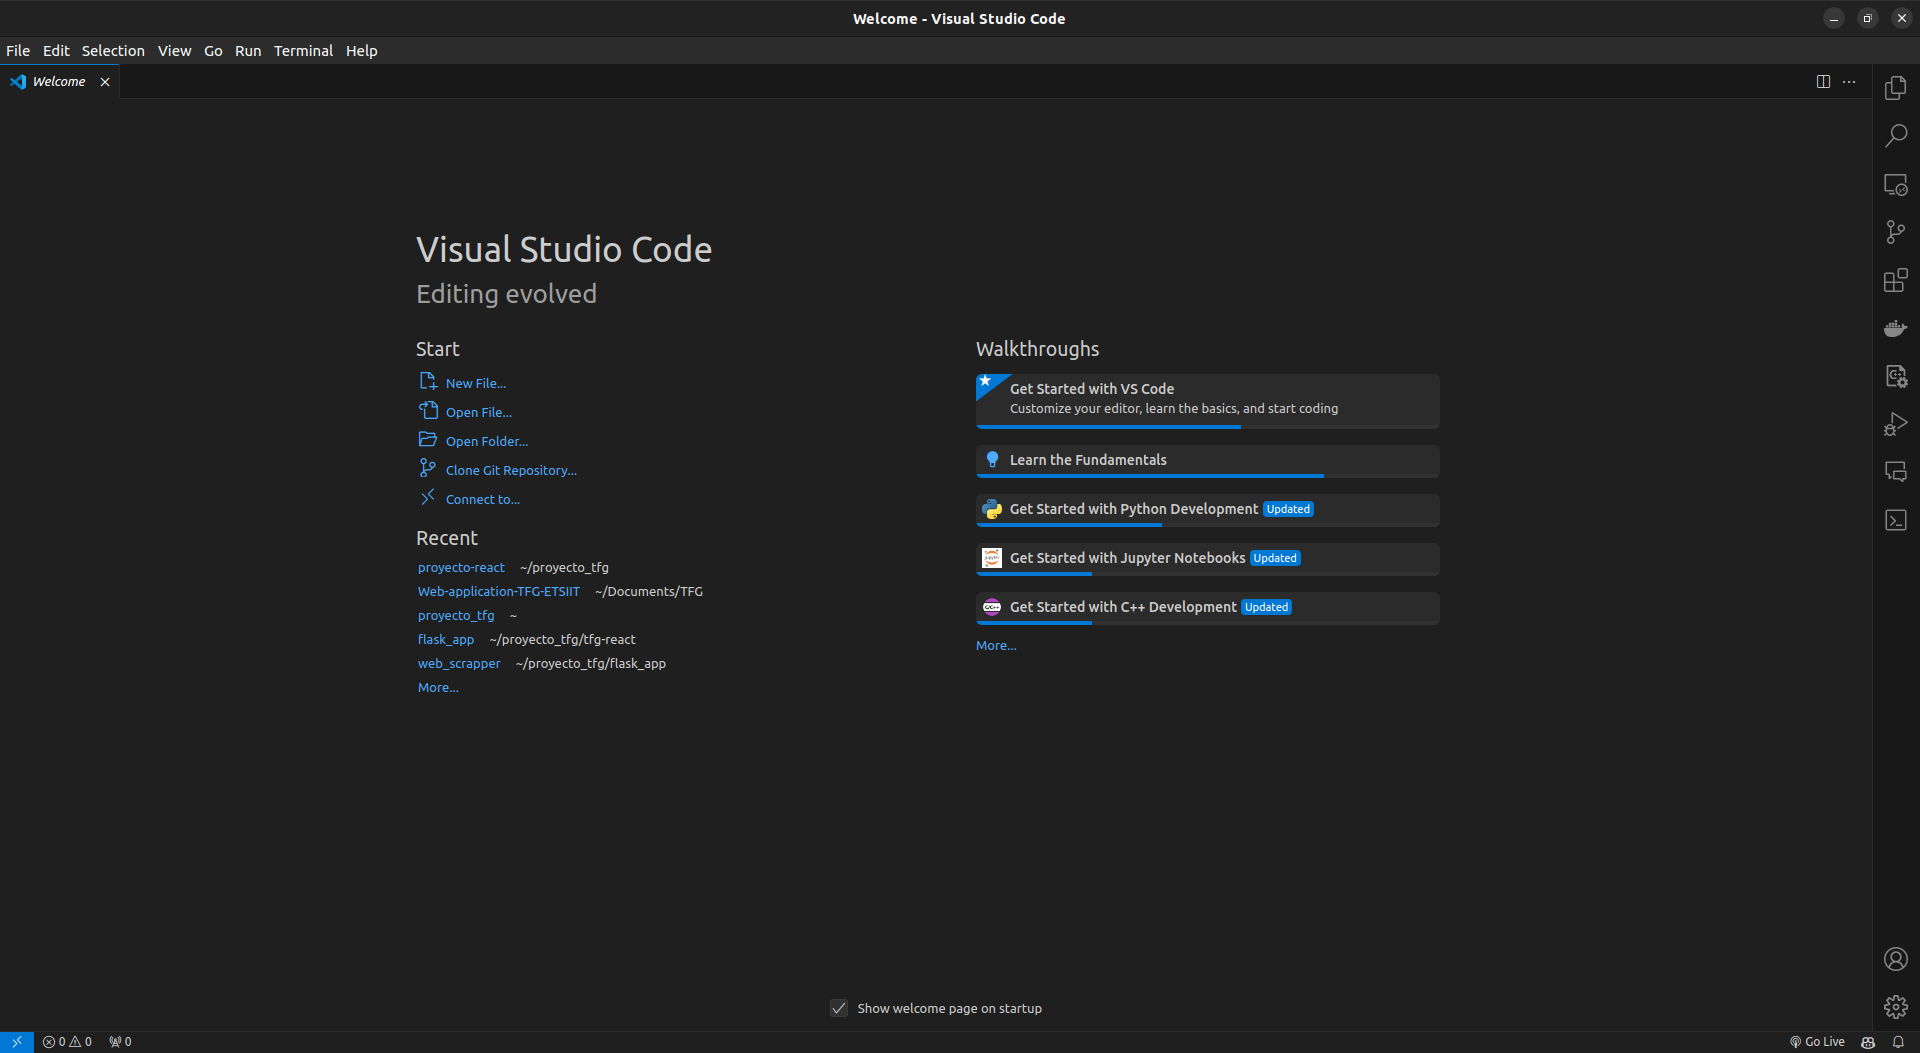
\includegraphics[width=1\textwidth]{./imagenes/vscode.png}
    \caption{Visual Studio.}
    \label{fig:vscode}
\end{figure}


La razón principal de la elección de Visual Studio Code es la familiaridad. He utilizado este editor desde que empecé mis estudios de grado y la personalización, extensiones, integración con Git y la facilidad de uso la hacen una herramienta tremendamente útil y versátil. Además, pueden integrarse terminales para ejecutar comandos y es multiplataforma, lo que permite trabajar en cualquier sistema operativo.\newline

\renewcommand{\icon}[1]{\includegraphics[height=18pt]{#1}}
\subsubsection*{SQLite Studio \protect\icon{./imagenes/sqlite_logo.png}}

SQLite Studio\footnote{\url{https://sqlitestudio.pl/}}(Figura \ref{fig:sqlitestudio}) es un administrador de bases de datos multiplataforma que permite navegar y editar archivos de bases de datos SQLite. Dispone de características como la creación de bases de datos, tablas, índices, vistas, procedimientos almacenados, funciones, etc. Además, permite ejecutar consultas SQL, importar y exportar datos, entre otras.\newline


La elección de SQLite Studio se debe a que es un administrador de bases de datos muy completo y fácil de usar. Permite gestionar varias bases de datos SQLite de forma sencilla y eficiente, lo que facilita el desarrollo y la depuración.\newline

\begin{figure}[H]
    \centering
    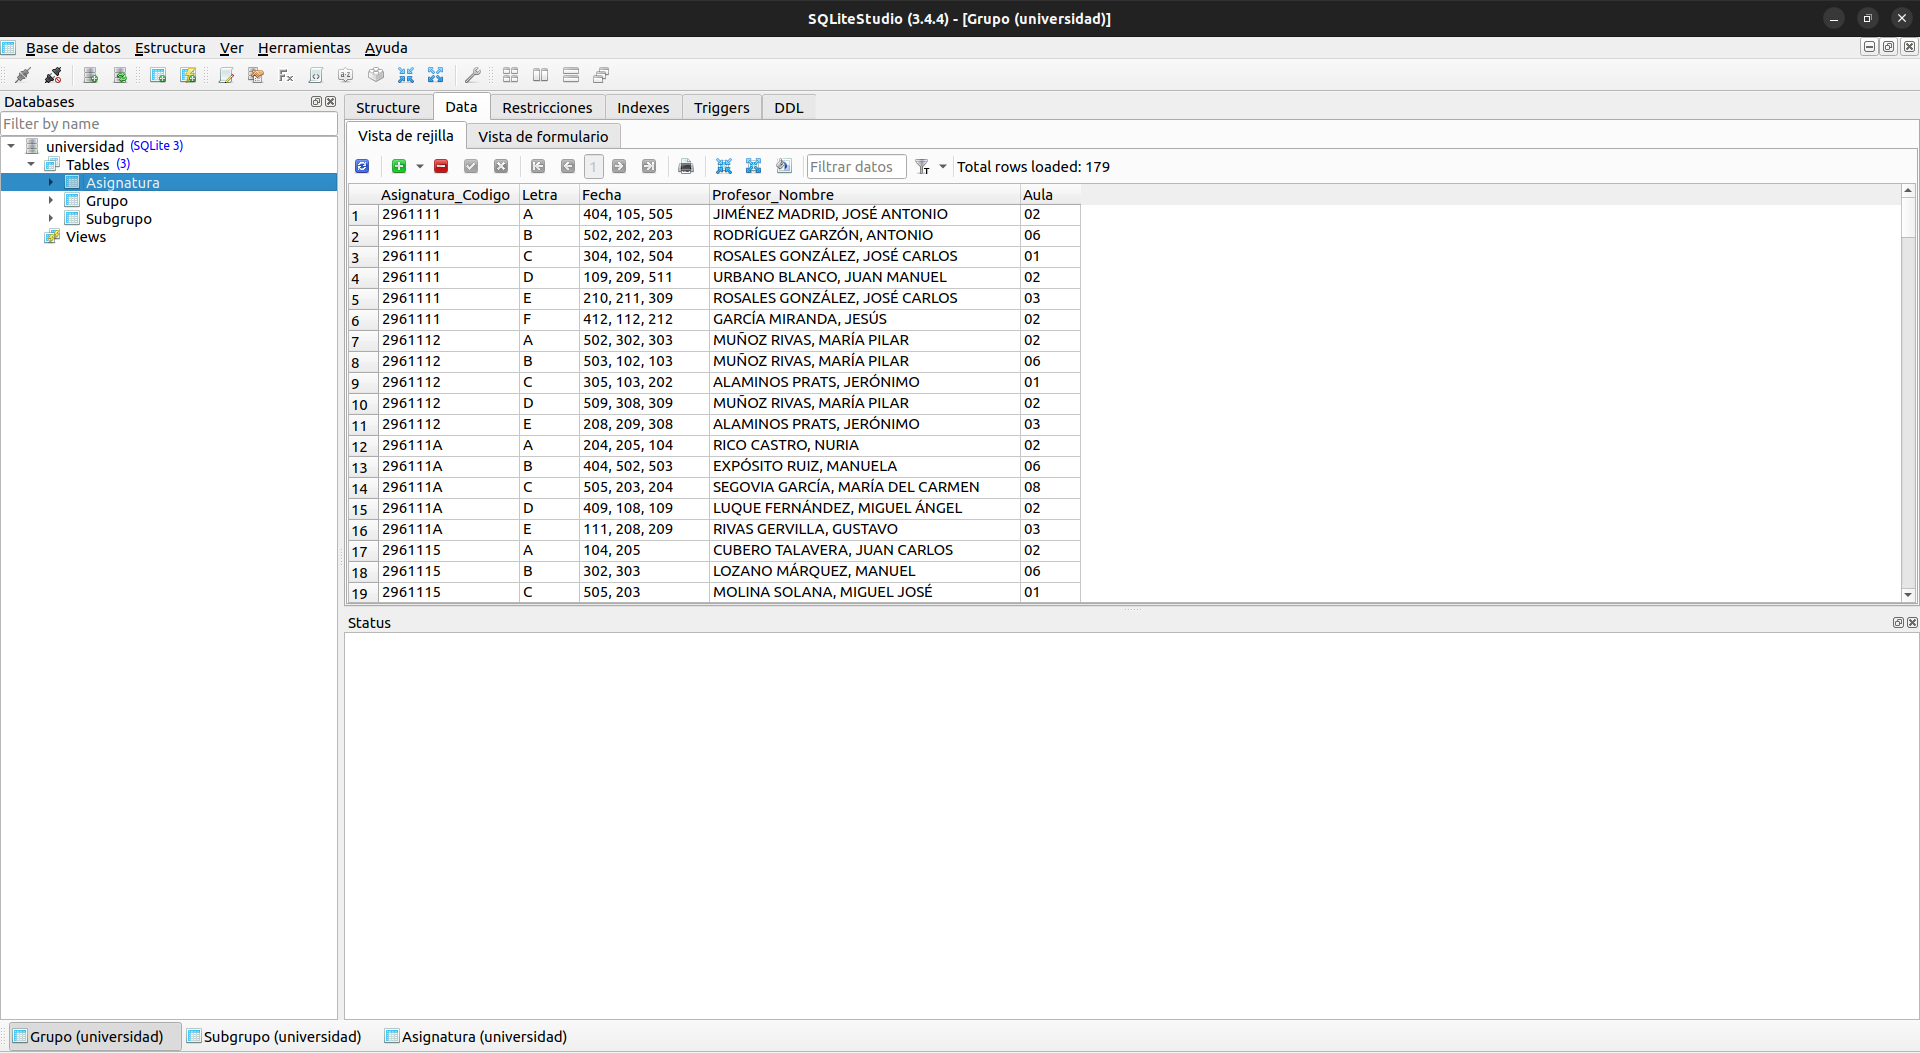
\includegraphics[width=1\textwidth]{./imagenes/SQLiteStudio.png}
    \caption{SQLite Studio.}
    \label{fig:sqlitestudio}
\end{figure}

\vspace{-1cm}

\renewcommand{\icon}[1]{\includegraphics[height=18pt]{#1}}
\subsubsection*{Postman \protect\icon{./imagenes/postman_logo.png}}

Postman\footnote{\url{https://www.postman.com/}}(Figura \ref{fig:postman}) es una plataforma para crear y utilizar API. Simplifica cada paso del ciclo de vida de una API y agiliza el desarrollo. Permite enviar solicitudes HTTP a un servidor y recibir respuestas. Dispone de características como la creación de \textit{colecciones de solicitudes}, la automatización de pruebas, la documentación de la API, entre otras. Es muy popular y cuenta con una gran cantidad de usuarios en todo el mundo.\newline

\begin{figure}[H]
    \centering
    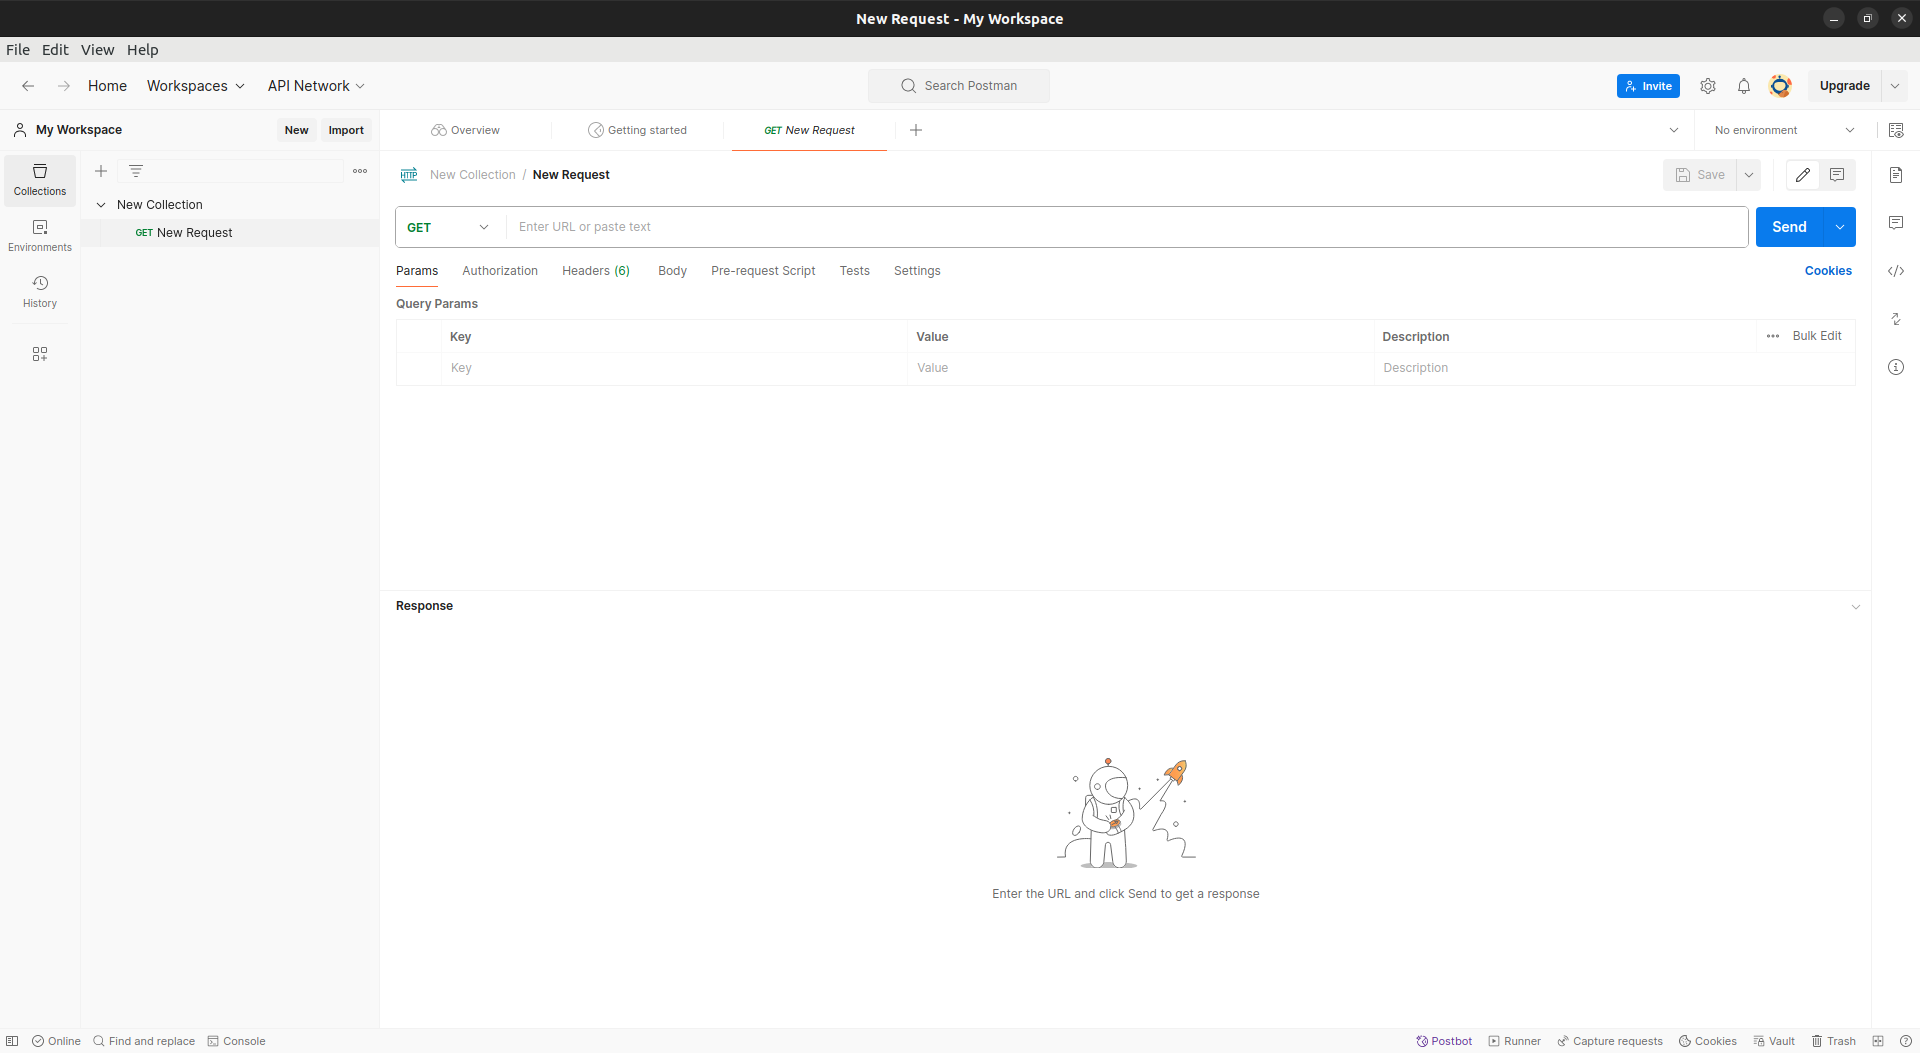
\includegraphics[width=1\textwidth]{./imagenes/postman.png}
    \caption{Postman.}
    \label{fig:postman}
\end{figure}

La elección de Postman se debe a una recomendación de mi tutor. Es una herramienta muy útil para probar API y asegurarse de que funcionan correctamente. Gracias a ella he podido probar los datos cruzados entre el backend y el frontend y depurar de manera más cómoda. Además, permite automatizar las pruebas y documentarlas.\newline


\section{Backend}
El backend es el encargado de administrar la funcionalidad general de la plataforma, operando en el servidor para procesar las solicitudes, manipular los datos y devolver la respuesta al cliente. En esta capa se almacena el código encargado de la lógica de negocio y la interacción con la base de datos. Su funcionalidad juega un papel esencial en la comunicación con el frontend y se asegura de que la información devuelta sea correcta, asegurando la integridad de los datos, el dinamismo y el diseño responsive de la interfaz de usuario. Actuando como núcleo funcional de la plataforma, se compone de las tecnologías que se detallan a continuación.\newline

En este apartado se describe la implementación del servicio Backend de la plataforma. Se especificará la estructura del código así como la implementación de la API mencionada en la sección de diseño y las tecnologías empleadas durante su desarrollo.\newline

\subsection{Servicios Web}

La integración del frontend con el backend se ha hecho por medio de botones en la interfaz de la plataforma. Al pulsar dichos botones se realizará una llamada HTTP al backend por medio de la biblioteca \textit{fetch}. Estos servicios se encargan de procesar las peticiones del cliente, realizar las operaciones necesarias en la base de datos y devolver la respuesta. A continuación, se detallan los servicios web implementados en la plataforma \textbf{GAC}:

\subsubsection*{Asignaturas}

Este servicio (Figura \ref{fig:get_asignaturas_curso}) es el encargado de obtener las asignaturas de un curso y cuatrimestre determinado por medio de una consulta SQL a la base de datos. Se hace por medio de una llamada GET con el siguiente endpoint de la Figura \ref{fig:get_asignaturas_endpoint}. Los datos de entrada son el \textbf{curso} y el \textbf{cuatrimestre} y la salida es un JSON con las asignaturas correspondientes a esos parámetros Figura \ref{fig:get_asignaturas_respuesta} y Figura \ref{fig:get_asignaturas_respuesta_cliente}.

\begin{figure}[H]
    \centering
    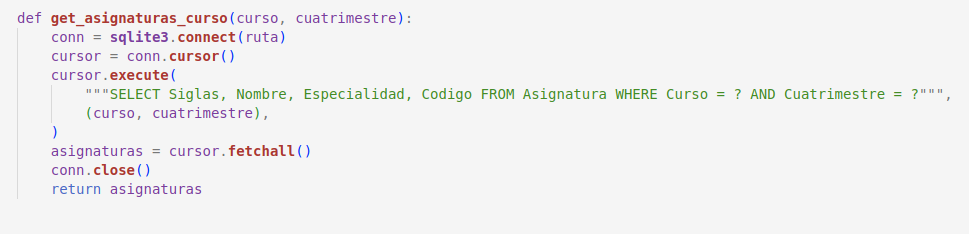
\includegraphics[width=1\textwidth]{./imagenes/get_asignaturas_curso.png}
    \caption{Servicio para obtener las asignaturas.}
    \label{fig:get_asignaturas_curso}
\end{figure}


\begin{figure}[H]
    \centering
    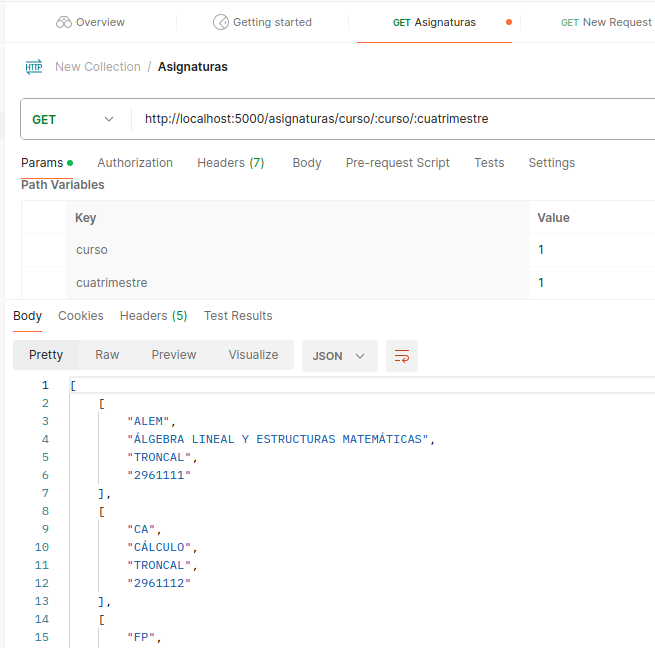
\includegraphics[width=1\textwidth]{./imagenes/get_asignaturas_respuesta.png}
    \caption{Respuesta servicio asignaturas.}
    \label{fig:get_asignaturas_respuesta}
\end{figure}

\begin{figure}[H]
    \centering
    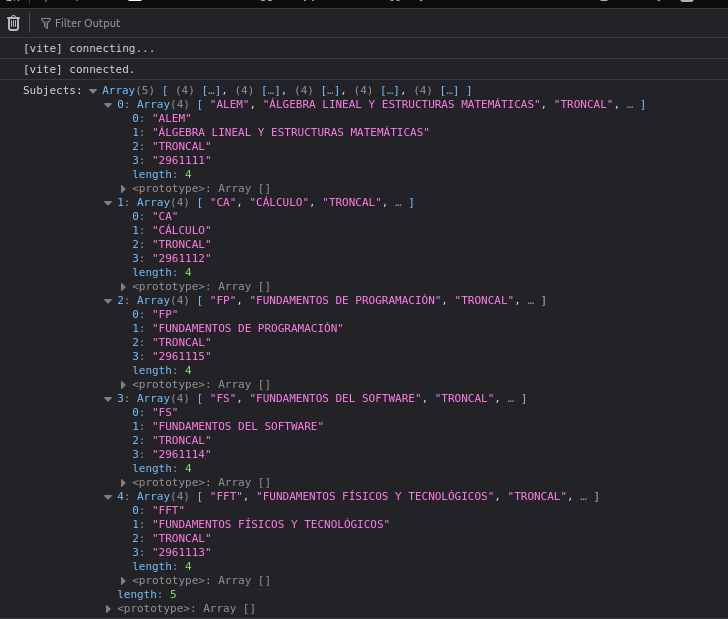
\includegraphics[width=1\textwidth]{./imagenes/get_asignaturas_respuesta_cliente.png}
    \caption{Respuesta servicio asignaturas en el cliente.}
    \label{fig:get_asignaturas_respuesta_cliente}
\end{figure}


\begin{figure}[H]
    \centering
    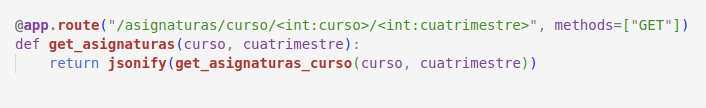
\includegraphics[width=1\textwidth]{./imagenes/get_asignaturas_endpoint.png}
    \caption{Endpoint servicio asignaturas.}
    \label{fig:get_asignaturas_endpoint}
\end{figure}

\subsection*{Grupos}

Este servicio (Figura \ref{fig:get_grupos_teoria}) es el encargado de obtener los grupos de teoría de una asignatura determinada por medio de una consulta SQL a la base de datos. Se hace por medio de una llamada GET con el siguiente endpoint de la Figura \ref{fig:get_grupos_teoria_endpoint}. Los datos de entrada son el \textbf{código} de la asignatura y la salida es un JSON con las asignaturas correspondientes a esos parámetros Figura \ref{fig:get_grupos_teoria_respuesta} y Figura \ref{fig:get_grupos_respuesta_cliente}.

\begin{figure}[H]
    \centering
    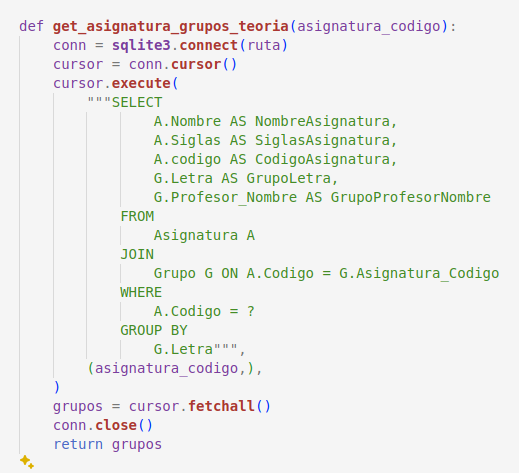
\includegraphics[width=0.8\textwidth]{./imagenes/get_grupos_teoria.png}
    \caption{Servicio para obtener los grupos de teoría.}
    \label{fig:get_grupos_teoria}
\end{figure}

\begin{figure}[H]
    \centering
    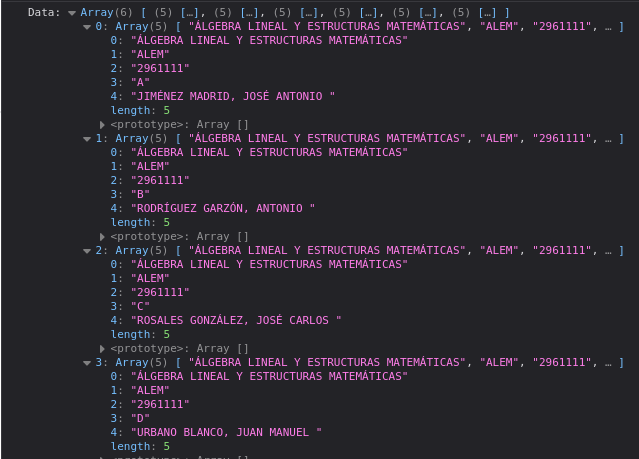
\includegraphics[width=0.9\textwidth]{./imagenes/get_grupos_teoria_respuesta_cliente.png}
    \caption{Respuesta servicio grupos en el cliente.}
    \label{fig:get_grupos_respuesta_cliente}
\end{figure}

\begin{figure}[H]
    \centering
    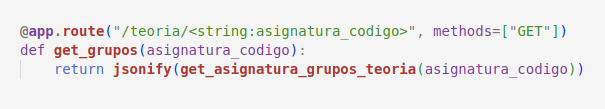
\includegraphics[width=1\textwidth]{./imagenes/get_grupos_teoria_endpoint.png}
    \caption{Endpoint servicio grupos.}
    \label{fig:get_grupos_teoria_endpoint}
\end{figure}

\begin{figure}[H]
    \centering
    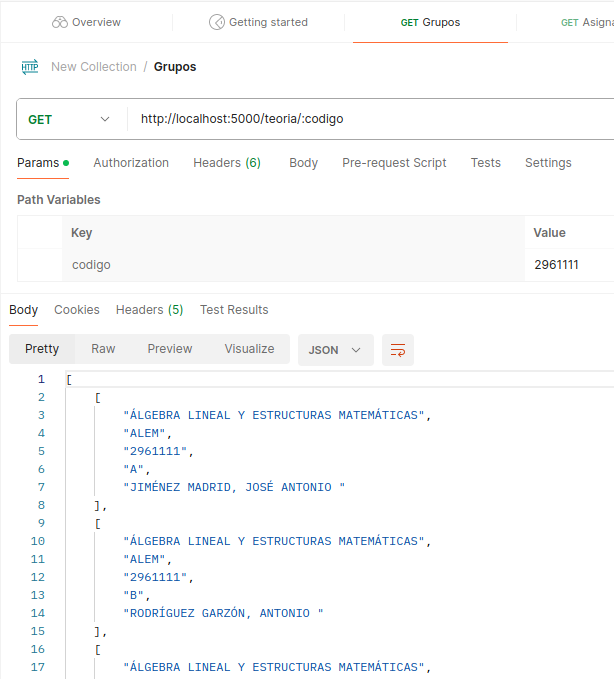
\includegraphics[width=0.8\textwidth]{./imagenes/get_grupos_teoria_respuesta.png}
    \caption{Respuesta servicio grupos.}
    \label{fig:get_grupos_teoria_respuesta}
\end{figure}


\subsection*{Subgrupos}

Este servicio (Figura \ref{fig:get_subgrupos}) es el encargado de obtener los subgrupos de prácticas de un grupo y asignatura determinada por medio de una consulta SQL a la base de datos. Se hace por medio de una llamada GET con el siguiente endpoint de la Figura \ref{fig:get_subgrupos_endpoint}. Los datos de entrada son el \textbf{código} de la asignatura y el \textbf{grupo} concatenados y salida es un JSON con el código de la asignatura y el subgrupo correspondiente a esos parámetros Figura \ref{fig:get_subgrupos_respuesta} y Figura \ref{fig:get_subgrupos_respuesta_cliente}.

\begin{figure}[H]
    \centering
    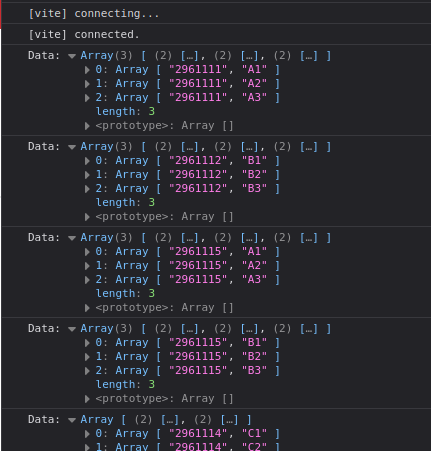
\includegraphics[width=0.8\textwidth]{./imagenes/get_subgrupos_respuesta_cliente.png}
    \caption{Respuesta serivicio subgrupos en el cliente.}
    \label{fig:get_subgrupos_respuesta_cliente}
\end{figure}

\begin{figure}[H]
    \centering
    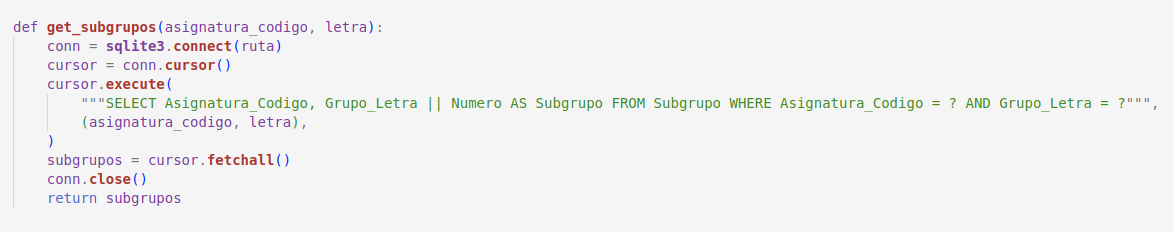
\includegraphics[width=1.1\textwidth]{./imagenes/get_subgrupos.png}
    \caption{Servicio para obtener los subgrupos de prácticas.}
    \label{fig:get_subgrupos}
\end{figure}

\begin{figure}[H]
    \centering
    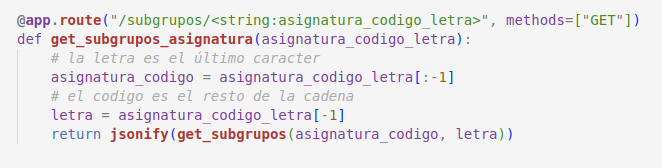
\includegraphics[width=1\textwidth]{./imagenes/get_subgrupos_endpoint.png}
    \caption{Endpoint servicio subgrupos.}
    \label{fig:get_subgrupos_endpoint}
\end{figure}

\begin{figure}[H]
    \centering
    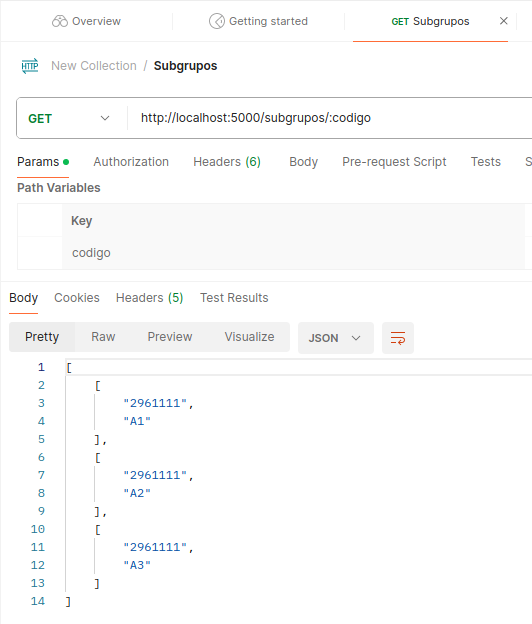
\includegraphics[width=0.8\textwidth]{./imagenes/get_subgrupos_respuesta.png}
    \caption{Respuesta servicio subgrupos.}
    \label{fig:get_subgrupos_respuesta}
\end{figure}

\subsection*{Horarios}

Este servicio (Figura \ref{fig:get_horarios} y Figura \ref{fig:get_fecha_grupo_subgrupo}) es el encargado de obtener las distintas combinaciones de grupos que conforman los horarios por medio de varias llamadas a funciones, en la sección 6.2.2 se explica en detalle su funcionamiento. Se hace por medio de una llamada GET con el siguiente endpoint de la Figura \ref{fig:get_horarios_endpoint}. Los datos de entrada son los \textbf{códigos} de las asignaturas y los \textbf{subgrupos} y salida es un JSON con los datos que conforman el horario de acuerdo a la estructura del componente \textbf{Calendario} que se explicará en la sección 6.3.1\ref{fig:get_horarios_respuesta} y Figura \ref{fig:get_horarios_respuesta_cliente}.

\begin{figure}[H]
    \centering
    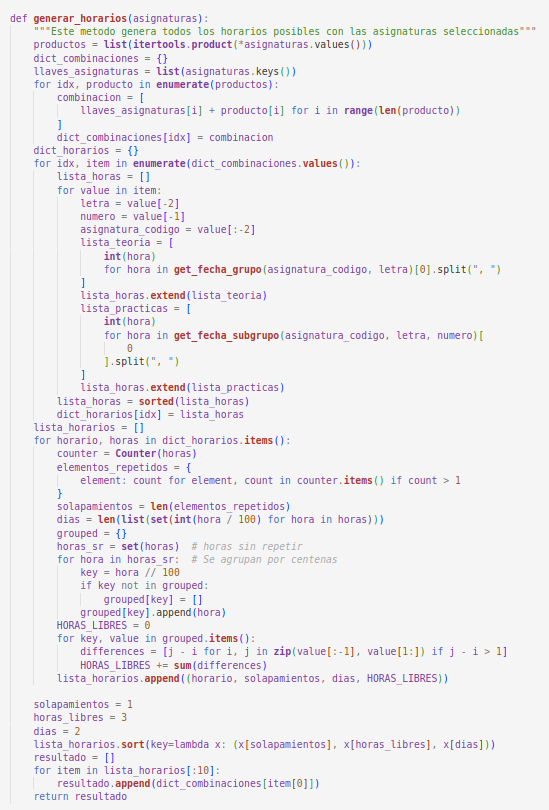
\includegraphics[width=0.95\textwidth]{./imagenes/get_horarios.png}
    \caption{Servicio para obtener los horarios.}
    \label{fig:get_horarios}
\end{figure}

\begin{figure}[H]
    \centering
    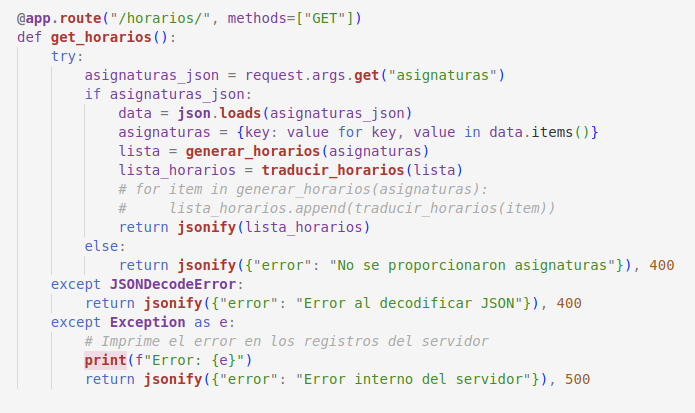
\includegraphics[width=1\textwidth]{./imagenes/get_horarios_endpoint.png}
    \caption{Endpoint servicio horarios.}
    \label{fig:get_horarios_endpoint}
\end{figure}

\begin{figure}[H]
    \centering
    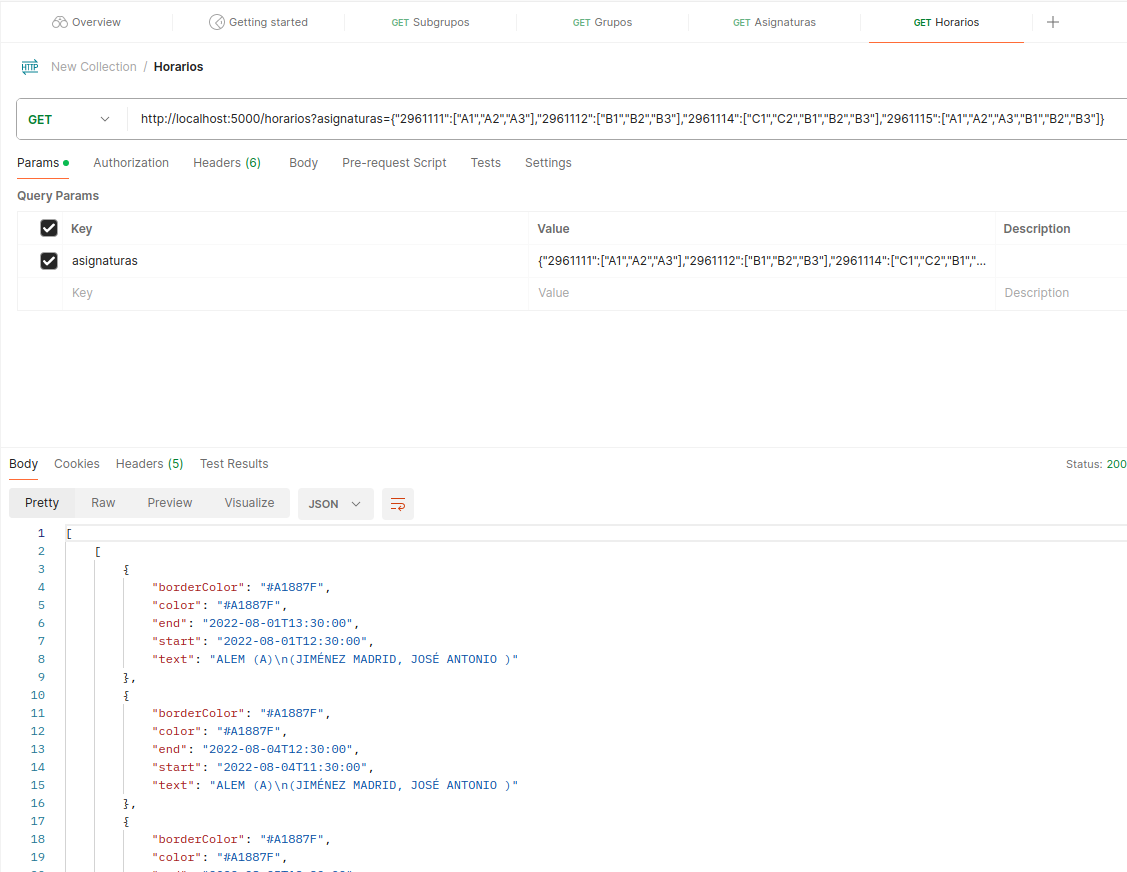
\includegraphics[width=1\textwidth]{./imagenes/get_horarios_respuesta.png}
    \caption{Respuesta servicio de horarios.}
    \label{fig:get_horarios_respuesta}
\end{figure}

\begin{figure}[H]
    \centering
    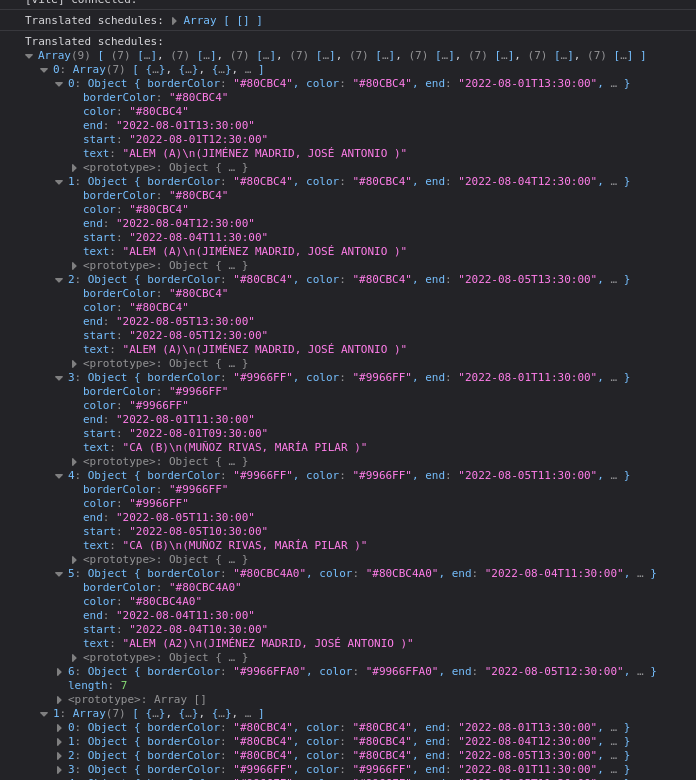
\includegraphics[width=0.8\textwidth]{./imagenes/get_horarios_respuesta_cliente.png}
    \caption{Respuesta servicio de horarios en el cliente.}
    \label{fig:get_horarios_respuesta_cliente}
\end{figure}

\begin{figure}[H]
    \centering
    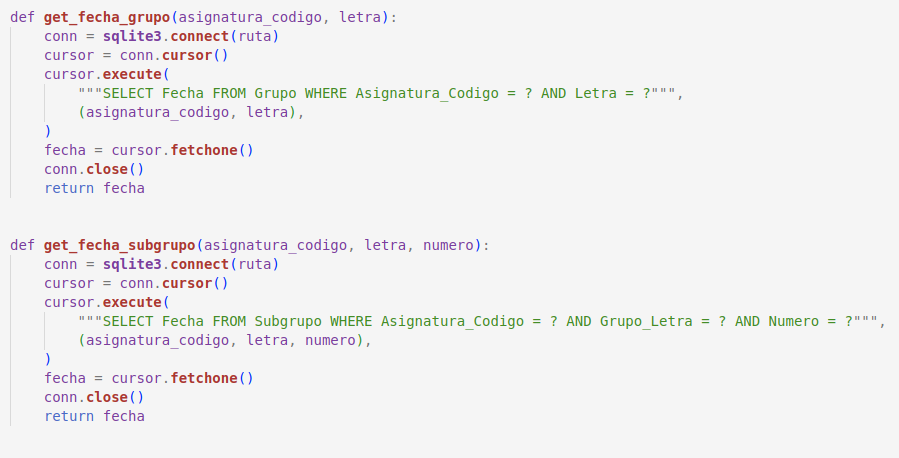
\includegraphics[width=1\textwidth]{./imagenes/get_fecha_grupo_subgrupo.png}
    \caption{Funciones usadas por el algoritmo de horarios.}
    \label{fig:get_fecha_grupo_subgrupo}
\end{figure}





\subsection{Algoritmo de Calendarios}

El algoritmo empleado para la creación de las combinaciones de grupos para los calendarios fue propuesto por \textbf{Jesús García Miranda}, secretario de la \textit{Escuela Técnica Superior de Ingenierías Informática y de Telecomunicaciones de la Universidad de Granada} con dirección de correo electrónico \href{mailto:jesusgm@ugr.es}{jesusgm@ugr.es}. Dada la complejidad de los algoritmos presentados en la sección 2, se optó por una solución que permitiera la creación de calendarios de forma rápida y sencilla.\newline

Antes de mostrar el pseudocódigo del algoritmo, téngase en cuenta que las horas de los grupos de las asignaturas se almacenan codificadas de la siguiente forma:\newline

El \textbf{día} de la semana se indica mediante las \textbf{centenas}, la \textbf{hora de inicio} de la clase se indica por medio de las \textbf{decenas y unidades}. Al ser 5 los días lectivos de la semana y 13 las horas que van desde el inicio de la jornada (8:30) hasta el final (20:00), una clase de 2 horas el lunes de 8:30 a 10:30 se codificaría como la secuencia de valores [101,102].\newline

\newpage

\begin{algorithm}[H]
    \caption{Generar Horarios}
    \label{alg:generar_horarios}
    \begin{algorithmic}[1]
        \Require Diccionario de asignaturas con sus subgrupos.
        \Ensure Lista de los 10 mejores horarios posibles.
        \Function{GenerarHorarios}{asignaturas}
            \State $productos$ = $asignaturas.prodCartesiano()$
            \State Concatear el código de asignatura a cada subgrupo de cada combinación.
            \State $diccionario-combinaciones$ = $productos$
            \State $horarios$ = $dict$
            \For{$combinacion$ en $productos$}
                \State $lista-horas$ = $[]$
                \For{$asignatura$ en $combinacion$}
                    \State $lista-horas$ = $get-teoria(asignatura)$
                    \State $lista-horas$ = $lista-horas$ $\cup$ $get-practicas(asignatura)$
                \EndFor
                \State $lista-horas.sort()$ \Comment{Se ordenan los números de las horas.}
                \State $horarios.append(lista-horas)$ \Comment{Cada horario está identificado.}
            \EndFor
            \State $horarios-evaluados$ = $dict$
            \For{$horario$ en $horarios$}
                \State $Key$ = $horario.getKey()$    \Comment{Se obtiene el identificador del horario.}
                \State $ponderacion$ = $[]$
                \State $ponderacion.append(contar-solapamientos(horario))$
                \State $ponderacion.append(contar-horas-muertas(horario))$
                \State $ponderacion.append(contar-dias-asistencia(horario))$
                \State $horarios-evaluados[Key]$ = $ponderacion$
            \EndFor
            \State $resultado$ = $[]$ 
            \State $horarios-evaluados.sort()$ \Comment{Se ordenan los por ponderación.}
            \For {$i$ en $range(10)$}
                \State $resultado.append(horarios[horarios-evaluados[i]])$
            \EndFor

            \Return $resultado$
        \EndFunction
    \end{algorithmic}
\end{algorithm}

\newpage

\subsection{Tecnologías utilizadas}

A continuación se detallan las tecnologías y librerías utilizadas en el desarrollo del backend.
% Para el desarrollo de la plataforma se compone de un backend y un frontend. El backend hace de servidor y es el que se encarga de responder a las peticiones por medio de una API desarrollada en Python con Flask y SQLite como base de datos. El frontend incluye la interfaz de usuario y ha sido desarrollada en ReactJS. A continuación se detallan las tecnologías utilizadas en detalle.\newline

% Para el desarrollo del backend se ha utilizado una arquitecura cliente-servidor basada en una arquitectura orientada a servicios (SOA).\newline

\renewcommand{\icon}[1]{\includegraphics[height=22pt]{#1}}
\subsubsection*{Pyhton \protect\icon{./imagenes/python_logo.png}}
Es un lenguaje de programación interpretado, orientado a objetos y de alto nivel con semántica dinámica. Su sintaxis es clara y legible, lo que facilita la escritura de código y la lectura del mismo. Es un lenguaje multiplataforma, lo que significa que se puede ejecutar en cualquier sistema operativo. Es versátil y se puede utilizar en una amplia variedad de aplicaciones, desde desarrollo web hasta análisis de datos y aprendizaje automático. Es un lenguaje de programación muy popular y cuenta con una gran cantidad de bibliotecas y marcos de trabajo que facilitan el desarrollo de aplicaciones \cite{python2021python}.\newline

El motivo de usar Python para el desarrollo del backend se debe a una elección personal, motivada por el interés de aprender un nuevo lenguaje de programación tan ampliamente utilizado a nivel mundial. Python es reconocido por su simplicidad y facilidad de uso, lo que lo convierte en una excelente opción para el desarrollo de aplicaciones web. Cuenta con una gran cantidad de bibliotecas y marcos de trabajo que facilitan el desarrollo de aplicaciones web, la documentación es extensa y la comunidad es muy activa y además soporta módulos y paquetes que lo que resulta en productos modulares y reutilizables.

\renewcommand{\icon}[1]{\includegraphics[height=20pt]{#1}}
\subsubsection*{Flask \protect\icon{./imagenes/flask_logo.png}}

Es un framework de aplicaciones web escrito en Python. Se compone de un núcleo WSGI\footnote{\url{https://wsgi.readthedocs.io/en/latest/}} simple y fácil de extender que permite a los desarrolladores crear aplicaciones web rápidamente con una mínima configuración. Flask\footnote{\url{https://pythonbasics.org/what-is-flask-python/}} es ligero y fácil de usar, lo que lo convierte en una muy buena opción para desarrollar proyectos de pequeños o medianos. Es muy popular y cuenta con una gran cantidad de bibliotecas y extensiones que facilitan el desarrollo \cite{grinberg2018flask}.\newline

La recomendación de usar Flask vino por parte de mi tutor, ya que es un framework muy popular, modular y fácil de usar. En la red hay disponibles una gran cantidad de guías que explican los pasos necesarios para hacer una configuración inicial y empezar a desarrollar aplicaciones. Dada la familiaridad con este framework y su baja curva de aprendizaje, se decidió utilizar para el desarrollo del backend.

\renewcommand{\icon}[1]{\includegraphics[height=18pt]{#1}}
\subsubsection*{SQLite \protect\icon{./imagenes/sqlite_logo.png}}

SQLite\footnote{\url{https://www.sqlite.org/index.html}} es una base de datos relacional embebida, de código abierto, que se implementa como una biblioteca de programación C. Es rápida, ligera y fácil de usar, lo que la convierte en una excelente opción para aplicaciones de pequeña o mediana envergadura. Es muy popular y cuenta con una gran cantidad de bibliotecas y extensiones que facilitan el desarrollo \cite{kreibich2010using}.\newline

La elección de SQLite como base de datos se debe a que es una base de datos embebida, lo que significa que no requiere un servidor de base de datos separado para funcionar. Esto simplifica la configuración y el despliegue de la plataforma. Además, es de tipo relacional, y dada la estructura rígida de asignaturas, grupos, subgrupos, aulas, etc., se ajusta perfectamente a las necesidades de la plataforma. Por último, es muy fácil de usar y cuenta con una gran cantidad de bibliotecas y extensiones que facilitan el desarrollo, como es el caso de \textbf{SQLAlchemy}\footnote{\url{https://www.sqlalchemy.org/}} que usaremos para facilitar la interacción con la base de datos.

\renewcommand{\icon}[1]{\includegraphics[height=20pt]{#1}}
\subsubsection*{Docker \protect\icon{./imagenes/docker_logo.png}}

Docker \footnote{\url{https://www.docker.com/}} es una tecnología de organización de contenedores que permite empaquetar aplicaciones en contenedores virtuales que pueden ejecutarse en cualquier lugar. Provee un tipo de virtualización más ligera que las máquinas virtuales tradicionales, ya que comparte el núcleo del sistema operativo con otros contenedores.\newline

El motivo de usar Docker es mi familiaridad con la herramienta y mi interés en aprender más sobre ella. Docker es una tecnología muy popular y ampliamente utilizada en la industria. Permite empaquetar aplicaciones en contenedores virtuales que pueden ejecutarse en las mismas condiciones independientemente del sistema operativo subyacente, lo que facilita la configuración y el despliegue de la plataforma. Además, es muy eficiente y ligero, permitiendo ejecutar múltiples contenedores en un mismo servidor.


\subsubsection*{Módulos utilizados}
\begin{itemize}
    \item \textbf{itertools:} Módulo con herramientas útiles para la creación de iteradores eficientes. Sus funciones para la creación de productos cartesianos y permutaciones han sido fundamentales para la creación de los horarios (Figura \ref{fig:get_horarios}).
    \item \textbf{sqlite3:} Módulo que permite la interacción con bases de datos SQLite. Se ha utilizado para realizar consultas SQL a la base de datos (Figuras \ref{fig:get_horarios}, \ref{fig:get_asignaturas_curso}, \ref{fig:get_grupos_teoria}, \ref{fig:get_subgrupos} y \ref{fig:get_fecha_grupo_subgrupo}).
    \item \textbf{json:} Módulo que permite la codificación y decodificación de objetos JSON. Se ha utilizado para devolver las respuestas en formato JSON (Figuras \ref{fig:get_horarios_respuesta}, \ref{fig:get_asignaturas_respuesta}, \ref{fig:get_grupos_teoria_respuesta} y \ref{fig:get_subgrupos_respuesta}).
\end{itemize}

\section{Frontend}

El frontend es la parte con la que el usuario final podrá interactuar. Hace de interfaz para las peticiones a la API, que son resueltas por el backend, donde se encuentra toda la lógica de la plataforma.\newline

La implementación del mismo se ha llevado a cabo utilizando la librería de React, que permite la creación de interfaces de usuario de forma sencilla y eficiente. La estructura se divide en componentes, que son elementos independientes que se encargan de mostrar la información y gestionar las interacciones con el usuario. Dichos componentes son la base de React y permiten la creación de aplicaciones escalables y fáciles de mantener.\newline

Todo este proceso se explica en detalle a continuación:\newline

\subsection{Componentes de React}

Son piezas de código reutilizable que renderizan una parte de la interfaz, pueden ser parametrizados, por medio de entradas llamadas ``props'' y pueden contener su propio estado. El estado es un objeto que contiene datos que pueden cambiar y se usan para controlar los cambios en la interfaz. Los componentes permiten componer interfaces más complejas a partir de elementos más sencillos, lo que facilita la escalabilidad y el mantenimiento.\newline


Para el desarrollo de la plataforma \textbf{GAC} se han desarrollado los siguientes componentes:

\begin{enumerate}
    \item \textbf{YearPanel:} Panel que muestra los cursos y cuatrimestres del grado seleccionado (Figura \ref{fig:yearpanel}).
    \begin{enumerate}
        \item \textbf{SelectorQuarter:} Selector que permite elegir el cuatrimestre.
        \item \textbf{SelectorYear:} Selector que permite elegir el curso.
    \end{enumerate}
    \item \textbf{SubjectPanel:} Panel que muestra las asignaturas del curso seleccionado (Figura \ref{fig:subjectPanel}). Interactúa con el componente \textbf{YearPanel} para obtener los datos y mostrarlos.
    \item \textbf{GroupPanel:} Panel que muestra los grupos de las asignaturas seleccionadas (Figura \ref{fig:groupPanel}). Interactúa con el componente \textbf{SubjectPanel} para obtener los datos y mostrarlos.
    \item \textbf{Calendar:} Cuadro que muestra los horarios de las asignaturas y grupos seleccionados (Figura \ref{fig:calendar}). Interactúa con el componente \textbf{GroupPanel} para obtener los datos y mostrarlos.
\end{enumerate}

\begin{figure}[H]
    \centering
    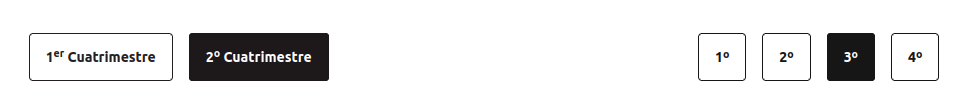
\includegraphics[width=1\textwidth]{./imagenes/year_panel.png}
    \caption{YearPanel.}
    \label{fig:yearpanel}
\end{figure}

\begin{figure}[H]
    \centering
    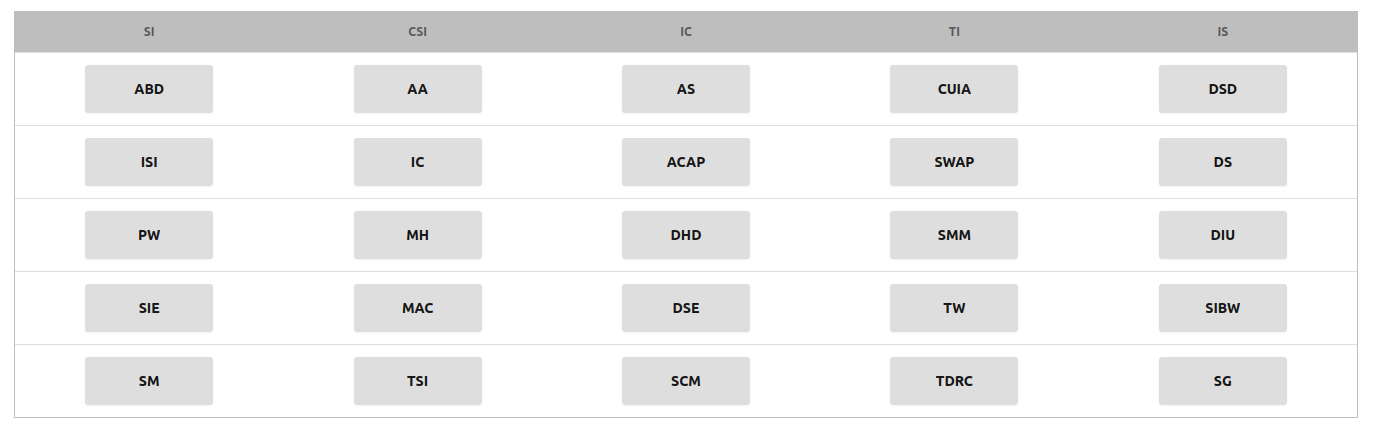
\includegraphics[width=1\textwidth]{./imagenes/subjects_panel.png}
    \caption{SubjectPanel.}
    \label{fig:subjectPanel}
\end{figure}

\begin{figure}[H]
    \centering
    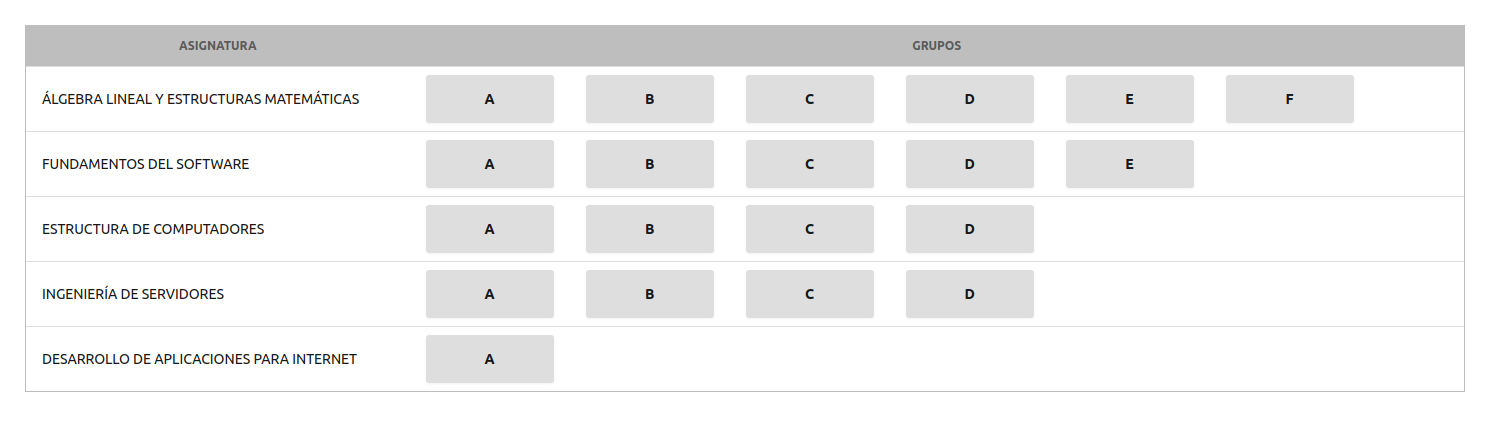
\includegraphics[width=1\textwidth]{./imagenes/group_panel.png}
    \caption{GroupPanel.}
    \label{fig:groupPanel}
\end{figure}

\begin{figure}[H]
    \centering
    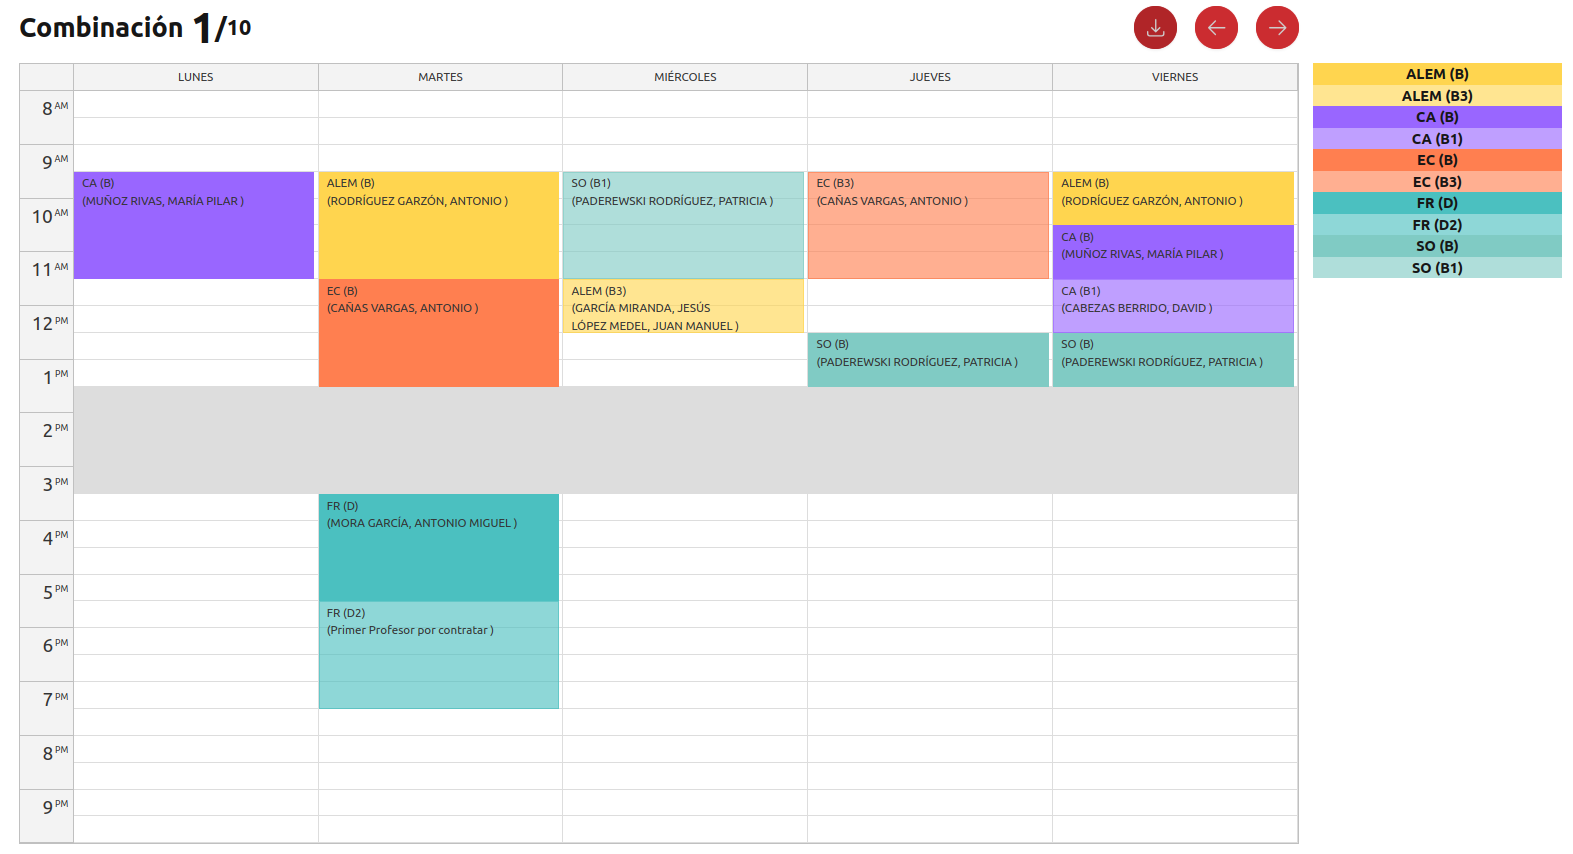
\includegraphics[width=1\textwidth]{./imagenes/calendar.png}
    \caption{Calendar.}
    \label{fig:calendar}
\end{figure}

\subsection{Herramientas utilizadas}

% El frontend es la parte de la plataforma con la que interactúan los usuarios finales. Es la capa de presentación e incluye todo aquello que el se ve. Juega un papel fundamental en la experiencia ya que es la primera impresión que se lleva el usuario y debe ser clara e intuitiva.\newline

\renewcommand{\icon}[1]{\includegraphics[height=22pt]{#1}}
\subsubsection*{React JS \protect\icon{./imagenes/react_logo.png}}

ReactJS\footnote{\url{https://es.reactjs.org/}} es una biblioteca de JavaScript de código abierto diseñada para crear interfaces de usuario interactivas, modulares y reutilizables. Permite el desarrollo de aplicaciones web que cambian sus datos sin necesidad de recargar la página. Provee un DOM mucho más eficiente y ligero almacenado en memoria y con el que interactúa en lugar de hacerlo directamente con el DOM del navegador. En la mayoría de webframeworks, se manipula el DOM completamente en cada uno de los eventos que desencadena la página, como consecuencia de esto, en los casos en los que se modifica una gran cantidad de datos, el rendimiento se ve seriamente afectado. ReactJS soluciona este problema, ya que solo modifica los elementos que han cambiado, haciendo uso de lo que se conoce como Virtual DOM\footnote{\url{https://es.reactjs.org/docs/faq-internals.html}}. Es muy popular y cuenta con una gran cantidad de bibliotecas y extensiones que facilitan el desarrollo \cite{aggarwal2018modern}.\newline

La utilización de ReactJS se debe a que es una biblioteca de JavaScript muy popular y ampliamente utilizada en la industria. Es muy eficiente y permite el desarrollo de aplicaciones web interactivas y modulares. Además, sirve de base para el desarrollo de aplicaciones móviles con React Native\footnote{\url{https://reactnative.dev/}}.\newline

Para ilustrar su popularidad, a continuación se muestra un gráfico con las tendencias de NPM\footnote{\url{https://npmtrends.com/@angular/core-vs-angular-vs-react-vs-vue}} que pese a no ser una fuente totalmente fiable (podemos ver un pico de Vue en la gráfica que puede haberse hecho por error o maliciosamente para alterar las estadísticas), nos da una idea de la popularidad de ReactJS en la actualidad.

\begin{figure}[H]
    \centering
    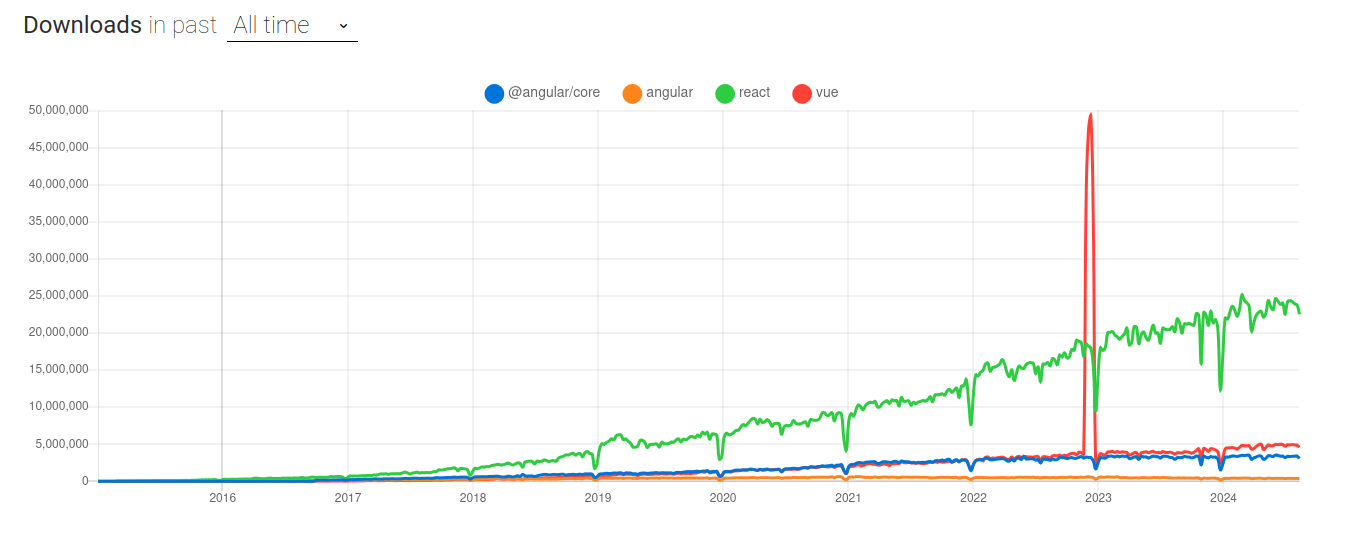
\includegraphics[width=1\textwidth]{./imagenes/Comparativa.png}
    \caption{Comparativa de descargas de frameworks de acuerdo a NPM.}
\end{figure}

\newpage

\subsection{Navegación}

Para la navegación por la plataforma existen dos tipos de usuarios, el usuario genérico (Figura \ref{fig:navegacion_sin_registro}) y el usuario registrado (Figura \ref{fig:navegacion_registro}). El usuario genérico puede acceder a la plataforma y visualizar los horarios de las asignaturas, mientras que el usuario registrado puede guardar los horarios y visualizarlos en cualquier momento.\newline

\subsubsection*{Navegación de usuario genérico}

\begin{figure}[H]
    \centering
    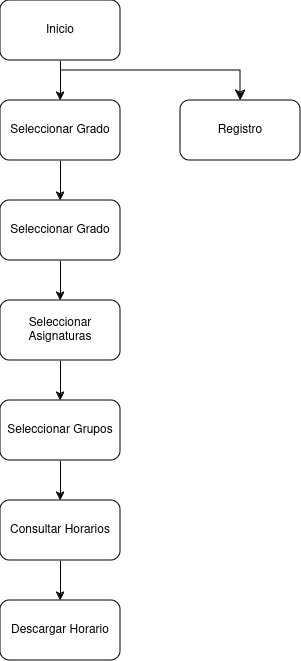
\includegraphics[width=0.5\textwidth]{./imagenes/Navegacion_sin_registro_Diagram.png}
    \caption{Navegación de usuario genérico.}
    \label{fig:navegacion_sin_registro}
\end{figure}

\subsubsection*{Navegación de usuario registrado}

\begin{figure}[H]
    \centering
    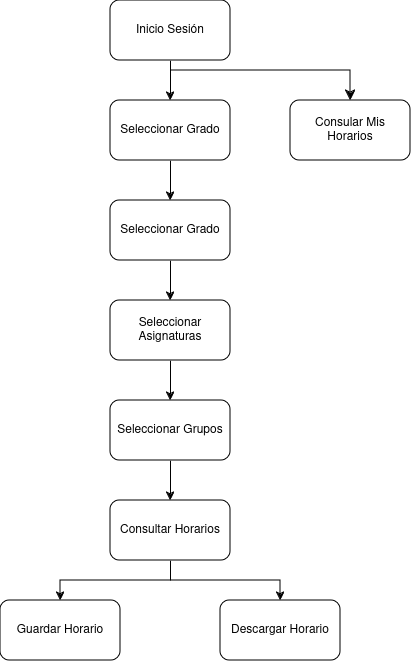
\includegraphics[width=0.6\textwidth]{./imagenes/Navegacion_Diagram.png}
    \caption{Navegación de usuario registrado.}
    \label{fig:navegacion_registro}
\end{figure}
